In this chapter, the visualization of objects whose positions have previously been computed (see Section ~\ref{ch:computation}) will be discussed. Also, the interaction patterns for the mobile application prototype will be defined.

\begin{itemize}
	\item \textbf {Visualization} - Describes how visualization is implemented in the App prototype.
	\item \textbf {User Interaction} - Lists information segments in the App prototype and possibilities of interaction for the user.
	\item \textbf {Removal of Node Overlapping} - Sketches the algorithm of how overlapping between multiple artist nodes are removed.
\end{itemize}

\section{Visualization}

After the computation of similarity measures and the resulting layout of music objects has been performed (see Section ~\ref{ch:computation}), the mode of visualization for the App prototype has to be defined. As has already been discussed, the possible modes of information display have been narrowed down due to several constraints, determining that a 2D visualization represents the best compromise for the scope of this thesis. Small screens on mobile devices introduce a further constraint: in most use cases, not all of the content will fit on one screen; therefore, a zooming and panning mechanism will be employed. To provide users with a rich experience, the objects shall not be shown as points, but as shapes - if an image of the object exists in an online source, it shall be used, or otherwise, a monocolored rectangle shall be shown. In order that users can orient themselves better, a non-solid background will be used - this provides visual feedback to the user while zooming when no objects are currently visible on the screen.

\begin{figure}[H]
  \centering
    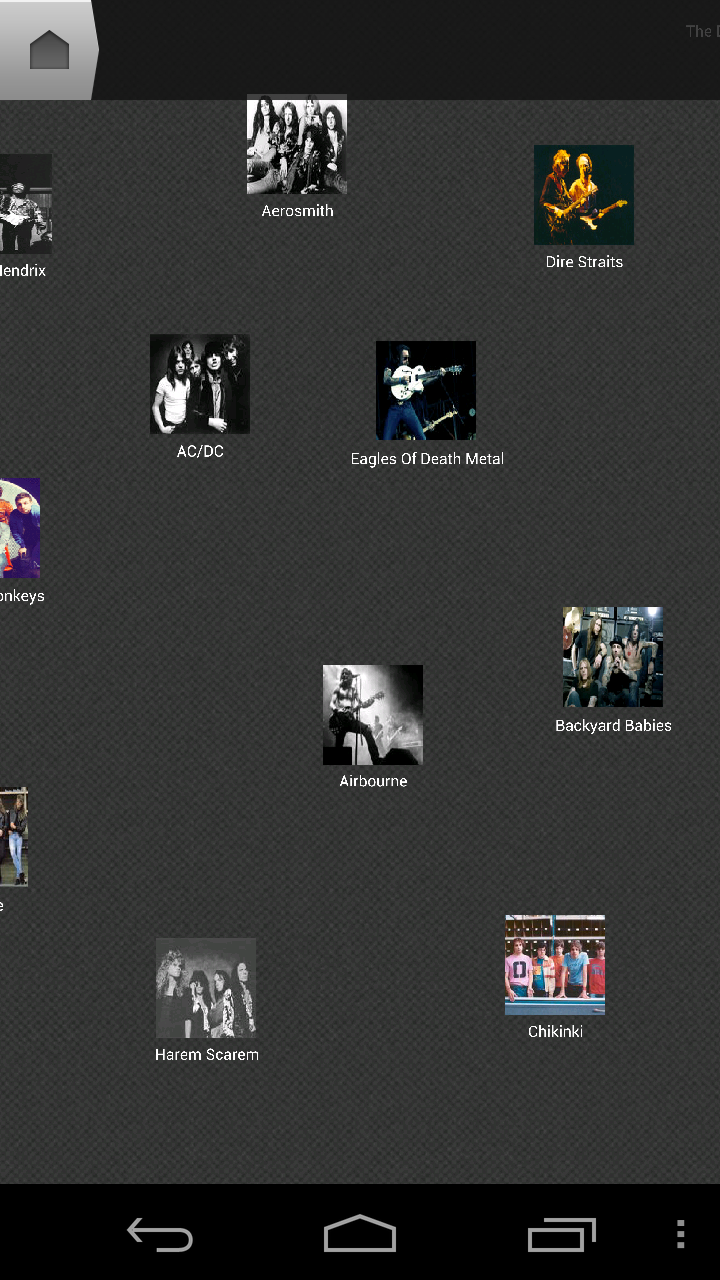
\includegraphics[width=0.4\textwidth]{figures/screen_mds_10_after_all_uncollided_nodes}
  \caption{Prototype Screenshot}
  \label{fig:prototype_screenshot}
\end{figure}

To let the reader grasp the previously described visualization, a screenshot of the prototype app is provided in Figure ~\ref{fig:prototype_screenshot}.

\section{User Interaction}

Information will be displayed to the user in a hierarchical way in the App prototype - to limit the amount of information displayed all at once, it is split up and logical links are established. The hierarchy is made up of:

\begin{itemize}
	\item \textbf{Artists} - images and labels with the names of the respective artists are displayed. Their positions relative to each other depict the artists' similarities. Here, the user can select an artist and proceed to the next hierarchical level by pressing a button:
	\item \textbf{A certain artist and her album(s)} - images and labels of the previously selected artist and her albums (stored on the device), arranged in a starlike way (without any similarity information conveyed). Again, the user can select an album and proceed to the next hierarchical level by pressing a button:
	\item \textbf{An album's tracks} - a list of tracks, carrying the image of the belonging album. The user can choose to start playback of one or all of the tracks.
	\item \textbf{Related Artists (Discovery)} - From within the \textbf{Artists} view, the user can choose to display artists which are related to a certain artist in a semantic way, as established by the Last.fm API.
	
\end{itemize}



To improve the user's understanding of the current navigational status, so-called breadcrumbs are introduced. The user can navigate within a two level hierarchy, where the higher level shows artists, and the lower level allows the user to view the albums of a previously selected artist. Breadcrumbs achieve "'visitor location awareness in a simple and direct way"' \cite{Tesoriero:2008:Breadcrumbs} if applied to 2D spaces. A breadcrumb in this context is a series of links displayed on top of the graph, each representing one hierarchical level. An example for breadcrumbs shown while a list of tracks (lowest hierarchical level) could be: "'Artist: Air > Album: Talkie Walkie"'. Further, a button is added which positions the viewport at the center of the graph, for the user to recover in case she has lost track of the viewport's position.

Within the graph viewport, interaction will be a mix of touch based interaction and hardware/software buttons, since most Android devices provide those affordances. Special accessibility functions for interaction without touch gestures are omitted since they would go beyond the scope of this thesis.
Following the established conventions of touch interfaces, controllable objects (like artists or albums) are made touchable. Likewise, the user can reach upper view hierarchies by pressing the back button.
Exploration of the graph is performed by two common touch gestures, namely pinch-to-zoom and one-finger-panning. To zoom, the user places two fingers on the graph viewport and moving her fingers either apart (zooming in) or towards each other (zooming out). To pan, the user places one finger on the graph and moves it around as if it were a piece of paper and the screen an aperture showing the paper.

\section{Removal of Node Overlapping}
\label{sec:removal-node-overlapping}

As the reader may have noticed, the positions of objects computed as described in Section ~\ref{ch:computation} don't respect any aesthetic criteria. ~\cite{Li:2005} gives an overview of such criteria, three of which also apply to graphs produced by MDS:

\begin{itemize}
	\item Minimization of the area taken up
	\item Minimization of total object distance
	\item Aspect ratio close to or matching the specification
\end{itemize}

However, an even more important aesthetic factor in the perception of graph drawings is the \textbf{removal of node overlappings}. The computational layout method applied in this thesis - spring model MDS (see Section ~\ref{ch:computation}) - can not give any heed to overlapping nodes (or margin between them), since nodes are positioned as points, not 2D objects. However, the objects do need to be displayed as 2D shapes (e.g. as rectangles, circles, images,...), and therefore the resulting layout can (and in many cases, will) contain overlappings.
As this may impact the perception of the graph by humans in a negative way (objects may even be completely hidden by other objects), a way has to be found to eliminate overlappings as reliably as possible, without affecting the conveyed information of object similarities too much.

The authors of ~\cite{journals/vlc/MisueELS95} therefore define the concept of the Mental Map, meaning that a graph has properties which should be maintained if transformed: Orthogonal Ordering, Proximity Relations, and Topology. An algorithm called Force Scan (FS) is then proposed to remove node overlappings while preserving the Mental Map of a graph. FS operates by first moving nodes horizontally, maintaining their horizontal ordering, and then moving nodes vertically, maintaining their vertical ordering. Several improvements to FS have been discussed (~\cite{Hayashi:1998:LAP:647550.728930} ~\cite{Huang03force-transfer:a} ~\cite{Li:2005}), while the algorithm in ~\cite{Huang03force-transfer:a} - \textbf{Force Transfer (FT)} - seems to be the most suitable for this thesis' use case, as it is of lower computational complexity than FS and produces pleasing layouts.

The FT algorithm identifies clusters of overlapping nodes, and then performs transfer scans on them: left-to-right, right-to-left, upside-to-downside, and downside-to-upside. During the scans, the nodes in each cluster are moved such that the clusters become free of overlaps. Multiple iterations may be necessary, as the separation of one cluster may cause nodes to move on top of nodes from other clusters - thereby forming new clusters. Finally, the layout eventually is overlap-free, preserving the aforementioned mental map of the graph.

The aforementioned methods of overlap-removal are complex (considering the need to form clusters), so the author decided to employ a more basic approach, but very similar to the previous algorithms. The graph canvas is virtually emptied, and re-filled one by one with the originally contained artist nodes, while making sure that a newly added node does not overlap with any others. The algorithm is described in the following listing:

\begin{enumerate}
\item Remove all nodes from the graph structure.	
\item For every node ("'subjectNode"') do:
	\begin{enumerate}
		\item For every node ("'alreadyPositionedNode"') in the set of already positioned nodes do:
		\item If the distance between subjectNode and alreadyPositionedNode is beloww a
		threshold, create a vector from alreadyPositionedNode's center to subjectNode's center, set
		its length such that they don't overlap, and displace subjectNode by it.
		\item If subjectNode still overlaps with another node, step to 2.a.
		\item Add subjectNode to the set of already positioned nodes.
	\end{enumerate}
\end{enumerate}

The result of this algorithm is a graph state which is free of node overlappings, with a predefined node rectangle size.

\section{Summary}

This chapter has made the concepts for visualization in the App prototype accessible to the reader. Apart from the introduction of implementation details regarding visualization (2D canvas for graph display, shape-based node rendering), the way how users interact with the prototype has been defined. Information is segmented into several contexts, "'breadcrumbs"' help the user navigate, and well-established multitouch gestures let the user control information presentation. 

As an improvement to readability and understandability of graph layouts, a computational method similar to force-transfer algorithms has been included in order to remove graph node overlappings.